\documentclass{standalone}
\usepackage{tikz}
\usetikzlibrary{patterns, positioning}


\begin{document}
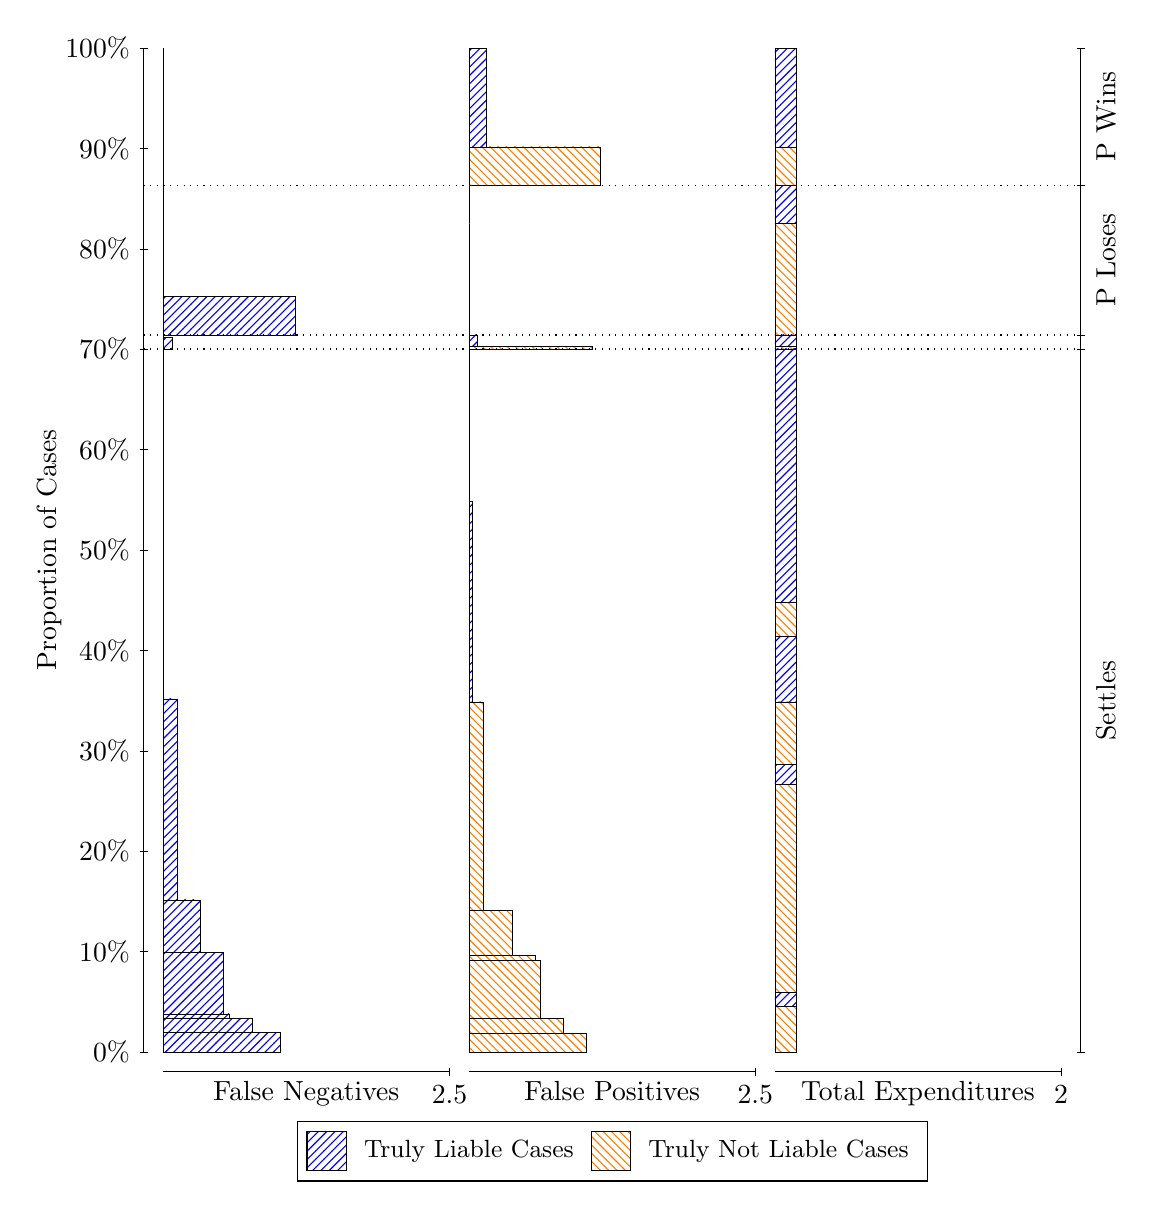
\begin{tikzpicture}
\draw[black, very thin] (1.5,1.75) -- (1.5,14.5);
\node[rotate=90, text=black, anchor=center] at (0.3, 8.125) {Proportion of Cases};
\draw[black, very thin] (1.45,1.75) -- (1.55,1.75);
\node[text=black, anchor=east] at (1.45, 1.75) {0\%};
\draw[black, very thin] (1.45,3.025) -- (1.55,3.025);
\node[text=black, anchor=east] at (1.45, 3.025) {10\%};
\draw[black, very thin] (1.45,4.3) -- (1.55,4.3);
\node[text=black, anchor=east] at (1.45, 4.3) {20\%};
\draw[black, very thin] (1.45,5.575) -- (1.55,5.575);
\node[text=black, anchor=east] at (1.45, 5.575) {30\%};
\draw[black, very thin] (1.45,6.85) -- (1.55,6.85);
\node[text=black, anchor=east] at (1.45, 6.85) {40\%};
\draw[black, very thin] (1.45,8.125) -- (1.55,8.125);
\node[text=black, anchor=east] at (1.45, 8.125) {50\%};
\draw[black, very thin] (1.45,9.4) -- (1.55,9.4);
\node[text=black, anchor=east] at (1.45, 9.4) {60\%};
\draw[black, very thin] (1.45,10.675) -- (1.55,10.675);
\node[text=black, anchor=east] at (1.45, 10.675) {70\%};
\draw[black, very thin] (1.45,11.95) -- (1.55,11.95);
\node[text=black, anchor=east] at (1.45, 11.95) {80\%};
\draw[black, very thin] (1.45,13.225) -- (1.55,13.225);
\node[text=black, anchor=east] at (1.45, 13.225) {90\%};
\draw[black, very thin] (1.45,14.5) -- (1.55,14.5);
\node[text=black, anchor=east] at (1.45, 14.5) {100\%};

\draw[black, very thin] (13.4,1.75) -- (13.4,14.5);
\draw[black, very thin] (13.35,1.75) -- (13.45,1.75);
\node[anchor=west] at (13.35, 1.75) {};
\draw[black, very thin] (13.35,10.678) -- (13.45,10.678);
\node[anchor=west] at (13.35, 10.678) {};
\draw[black, very thin] (13.35,10.856) -- (13.45,10.856);
\node[anchor=west] at (13.35, 10.856) {};
\draw[black, very thin] (13.35,12.758) -- (13.45,12.758);
\node[anchor=west] at (13.35, 12.758) {};
\draw[black, very thin] (13.35,14.5) -- (13.45,14.5);
\node[anchor=west] at (13.35, 14.5) {};

\draw[black, very thin, pattern color=blue, pattern=north east lines] (1.75,1.75) rectangle (3.2397,2.0016);
\draw[black, very thin, pattern color=blue, pattern=north east lines] (1.75,2.0016) rectangle (2.8763,2.1779);
\draw[black, very thin, pattern color=blue, pattern=north east lines] (1.75,2.1779) rectangle (2.5857,2.2345);
\draw[black, very thin, pattern color=blue, pattern=north east lines] (1.75,2.2345) rectangle (2.513,3.0123);
\draw[black, very thin, pattern color=blue, pattern=north east lines] (1.75,3.0123) rectangle (2.2223,3.6824);
\draw[black, very thin, pattern color=blue, pattern=north east lines] (1.75,3.6824) rectangle (1.9317,6.233);
\draw[black, very thin, pattern color=orange, pattern=north west lines] (1.75,6.233) rectangle (1.75,10.678);
\draw[black, very thin, pattern color=blue, pattern=north east lines] (1.75,10.678) rectangle (1.859,10.828);
\draw[black, very thin, pattern color=orange, pattern=north west lines] (1.75,10.828) rectangle (1.75,10.856);
\draw[black, very thin, pattern color=blue, pattern=north east lines] (1.75,10.856) rectangle (3.4213,11.343);
\draw[black, very thin, pattern color=orange, pattern=north west lines] (1.75,11.343) rectangle (1.75,12.758);
\draw[black, very thin, pattern color=orange, pattern=north west lines] (1.75,12.758) rectangle (1.75,13.245);
\draw[black, very thin, pattern color=blue, pattern=north east lines] (1.75,13.245) rectangle (1.75,14.5);
\draw[black, very thin, pattern color=orange, pattern=north west lines] (5.6333,1.75) rectangle (7.123,1.9876);
\draw[black, very thin, pattern color=orange, pattern=north west lines] (5.6333,1.9876) rectangle (6.8323,2.1779);
\draw[black, very thin, pattern color=orange, pattern=north west lines] (5.6333,2.1779) rectangle (6.5417,2.9179);
\draw[black, very thin, pattern color=orange, pattern=north west lines] (5.6333,2.9179) rectangle (6.469,2.9744);
\draw[black, very thin, pattern color=orange, pattern=north west lines] (5.6333,2.9744) rectangle (6.1783,3.5529);
\draw[black, very thin, pattern color=orange, pattern=north west lines] (5.6333,3.5529) rectangle (5.815,6.1953);
\draw[black, very thin, pattern color=blue, pattern=north east lines] (5.6333,6.1953) rectangle (5.6697,8.7459);
\draw[black, very thin, pattern color=blue, pattern=north east lines] (5.6333,8.7459) rectangle (5.6333,10.678);
\draw[black, very thin, pattern color=orange, pattern=north west lines] (5.6333,10.678) rectangle (7.1957,10.706);
\draw[black, very thin, pattern color=blue, pattern=north east lines] (5.6333,10.706) rectangle (5.7423,10.856);
\draw[black, very thin, pattern color=orange, pattern=north west lines] (5.6333,10.856) rectangle (5.6333,12.271);
\draw[black, very thin, pattern color=blue, pattern=north east lines] (5.6333,12.271) rectangle (5.6333,12.758);
\draw[black, very thin, pattern color=orange, pattern=north west lines] (5.6333,12.758) rectangle (7.3047,13.245);
\draw[black, very thin, pattern color=blue, pattern=north east lines] (5.6333,13.245) rectangle (5.8513,14.5);
\draw[black, very thin, pattern color=orange, pattern=north west lines] (9.5167,1.75) rectangle (9.7892,2.3285);
\draw[black, very thin, pattern color=blue, pattern=north east lines] (9.5167,2.3285) rectangle (9.7892,2.5048);
\draw[black, very thin, pattern color=orange, pattern=north west lines] (9.5167,2.5048) rectangle (9.7892,5.1472);
\draw[black, very thin, pattern color=blue, pattern=north east lines] (9.5167,5.1472) rectangle (9.7892,5.3988);
\draw[black, very thin, pattern color=orange, pattern=north west lines] (9.5167,5.3988) rectangle (9.7892,6.1953);
\draw[black, very thin, pattern color=blue, pattern=north east lines] (9.5167,6.1953) rectangle (9.7892,7.0297);
\draw[black, very thin, pattern color=orange, pattern=north west lines] (9.5167,7.0297) rectangle (9.7892,7.4576);
\draw[black, very thin, pattern color=blue, pattern=north east lines] (9.5167,7.4576) rectangle (9.7892,10.678);
\draw[black, very thin, pattern color=orange, pattern=north west lines] (9.5167,10.678) rectangle (9.7892,10.706);
\draw[black, very thin, pattern color=blue, pattern=north east lines] (9.5167,10.706) rectangle (9.7892,10.856);
\draw[black, very thin, pattern color=orange, pattern=north west lines] (9.5167,10.856) rectangle (9.7892,12.271);
\draw[black, very thin, pattern color=blue, pattern=north east lines] (9.5167,12.271) rectangle (9.7892,12.758);
\draw[black, very thin, pattern color=orange, pattern=north west lines] (9.5167,12.758) rectangle (9.7892,13.245);
\draw[black, very thin, pattern color=blue, pattern=north east lines] (9.5167,13.245) rectangle (9.7892,14.5);
\draw[black, dotted] (1.5,10.678) -- (13.4,10.678);
\draw[black, dotted] (1.5,10.856) -- (13.4,10.856);
\draw[black, dotted] (1.5,12.758) -- (13.4,12.758);
\draw[black, very thin] (1.75,1.5) -- (5.3833,1.5);
\node[text=black, anchor=north] at (3.5667, 1.5) {False Negatives};
\draw[black, very thin] (5.3833,1.45) -- (5.3833,1.55);
\node[text=black, anchor=north] at (5.3833, 1.45) {2.5};

\draw[black, very thin] (5.6333,1.5) -- (9.2667,1.5);
\node[text=black, anchor=north] at (7.45, 1.5) {False Positives};
\draw[black, very thin] (9.2667,1.45) -- (9.2667,1.55);
\node[text=black, anchor=north] at (9.2667, 1.45) {2.5};

\draw[black, very thin] (9.5167,1.5) -- (13.15,1.5);
\node[text=black, anchor=north] at (11.333, 1.5) {Total Expenditures};
\draw[black, very thin] (13.15,1.45) -- (13.15,1.55);
\node[text=black, anchor=north] at (13.15, 1.45) {2};

\node[text=black, centered, rotate=90] at (13.72, 6.2142) {Settles};

\node[text=black, centered, rotate=90] at (13.72, 11.807) {P Loses};
\node[text=black, centered, rotate=90] at (13.72, 13.629) {P Wins};

\draw (7.449999999999999,1.5) node[draw=none] (baseCoordinate) {};
\begin{scope}[align=center]
        \matrix[scale=0.5, draw=black, below=0.5cm of baseCoordinate, nodes={draw}, column sep=0.1cm]{
            \node[rectangle, draw, minimum width=0.5cm, minimum height=0.5cm, pattern color=blue, pattern=north east lines] {}; &
            \node[draw=none, font=\small, text=black] (B) {Truly Liable Cases}; &
            \node[rectangle, draw, minimum width=0.5cm, minimum height=0.5cm, pattern color=orange, pattern=north west lines] {}; &
            \node[draw=none, font=\small, text=black] (B) {Truly Not Liable Cases}; \\
            };
\end{scope}

\end{tikzpicture}
\end{document}